\documentclass{article}
\usepackage[a4paper, total={6in, 8in}]{geometry}
\usepackage[utf8]{inputenc}
\frenchspacing

% ------------------------------------------------------------
\usepackage{caption}
\captionsetup{labelformat=empty,labelsep=none}
\usepackage{scalerel,stackengine,amsmath}
\usepackage{mathtools}
\usepackage{dsfont}
\usepackage{multicol}
\usepackage{algorithm2e}
\usepackage{amsfonts}
\usepackage{enumerate}
\usepackage{enumitem}
% ------------------------------------------------------------

% image
\newcommand{\incl}[2]{\includegraphics[width=#1\textwidth]{#2}}
\newcommand{\inclc}[2]{\begin{center}\includegraphics[width=#1\textwidth]{#2}\end{center}}
% description
\newcommand{\thetitle}{}
\newcommand{\thecontents}{}
\newcommand{\thedate}{}
\newcommand{\theauthor}{}
\newcommand{\thedescription}{
	\section*{\thetitle}
	\begin{tabular}{ll}%
	Inhalt:&\thecontents\\%
	Datum:&\thedate\\%
	Author:&\theauthor\\%
	\end{tabular}%
}
% -- math mode stuff
\newcommand{\meq}[1]{\begin{equation*}\begin{aligned}#1\end{aligned}\end{equation*}}
% \newcommand{\NN}{\mathbb{N}}
\newcommand{\NN}{\mathbb{N}}
\newcommand{\ZZ}{\mathbb{Z}}
\newcommand{\QQ}{\mathbb{Q}}
\newcommand{\RR}{\mathbb{R}}
\newcommand{\CC}{\mathbb{C}}
\newcommand{\subt}[1]{\normalfont{(#1)}}
\newcommand{\ifcases}[2]{\begin{equation*}#1\begin{cases}#2\end{cases}\end{equation*}}
\newcommand{\ring}[1]{(#1,+,\cdot)}
\newcommand{\estimates}{\mathrel{\hat{=}}}
\newcommand{\OO}{\mathcal{O}}
\newcommand{\LRA}{\Leftrightarrow}
\newcommand{\LA}{\Leftarrow}
\newcommand{\RA}{\Rightarrow}
\newcommand{\textabove}[2]{\mathrel{\stackrel{\makebox[0pt]{\mbox{\normalfont\tiny #1}}}{#2}}}
\newcommand{\myqed}[1]{\hfill$\Box${\footnotesize#1}}
\newcommand{\neo}[1]{\begin{pmatrix}#1\end{pmatrix}}
\newcommand{\SsS}{\mathcal{S}}
\newcommand{\correct}{\hfill\checkmark}
\newcommand{\ubr}[2]{\underbrace{#1}_{\mathclap{\text{#2}}}}
\newcommand{\obr}[2]{\overbrace{#1}^{\mathclap{\text{#2}}}}
\renewcommand{\star}{^*}
\newcommand{\blank}{\ttt{\textvisiblespace}}
\newcommand\equalhat{\mathrel{\stackon[1.5pt]{=}{\stretchto{%
    \scalerel*[\widthof{=}]{\wedge}{\rule{1ex}{3ex}}}{0.5ex}}}}
\newcommand{\correspondsto}{\equalhat}
\newcommand{\weg}{(weggelassen)}
\newcommand{\chf}{\mathds{1}}
	% -- enumerations
\newcommand{\abc}[1]{\begin{enumerate}[label=\alph*.]#1\end{enumerate}}
\newcommand{\num}[1]{\begin{enumerate}[label=\arabic*.]#1\end{enumerate}}
\newcommand{\bul}[1]{\begin{itemize}#1\end{itemize}}
% -- text mode stuff
% \newcommand{\note}[1]{(\textit{#1})}
\newcommand{\ttt}{\texttt}
\newcommand{\tbf}{\textbf}
\newcommand{\tit}{\textit}
\newcommand{\trt}{\textit}
\newcommand{\tsc}{\textsc}
\newcommand{\tul}{\underline}
\newcommand{\tsub}[1]{\tre{\large#1}}
% -- text input stuff
\newcommand{\ditto}{''}
% <warning_emoji>
\newcommand*{\TakeFourierOrnament}[1]{{%
\fontencoding{U}\fontfamily{futs}\selectfont\char#1}}
\newcommand*{\warning}{\TakeFourierOrnament{66}}
\newcommand{\warn}{{\Large\warning}\ \ }
% </warning_emoji>
% logic stuff
\newcommand{\tttrue}{\ttt{true}}
\newcommand{\fffalse}{\ttt{false}}
% algorithm stuff:
\newcommand{\wwhile}{\textbf{while}}
\newcommand{\ffor}{\textbf{for}}
\newcommand{\ggoto}{\textbf{goto}}
\newcommand{\ddo}{\textbf{do}}
\newcommand{\iif}{\textbf{if}}
\newcommand{\tthen}{\textbf{then}}
\newcommand{\eelse}{\textbf{else}}
\newcommand{\eend}{\textbf{end}}
\newcommand{\hhalt}{\textbf{halt}}
\newcommand{\aand}{\textbf{and}}
\newcommand{\oor}{\textbf{or}}
\newcommand{\ffunction}{\textbf{function}}
\newcommand{\rreturn}{\textbf{return}}
\newcommand{\cccc}{\hphantom{cccc}}
\newcommand{\ccc}{\hphantom{ccc}}
\newcommand{\cc}{\hphantom{cc}}
\renewcommand{\;}{;\\}
\newcommand{\cmt}[1]{\ttt{#1}}
\newcommand{\lims}{\limsup_{n\to\infty}}
\newcommand{\limi}{\liminf_{n\to\infty}}
\newcommand{\true}{\ttt{true}}
\newcommand{\false}{\ttt{false}}


% <local>
\usepackage{hyperref}
\usepackage{tikz}
\usepackage{titlesec}
% --------
\newcommand{\pickl}[1]{\begin{center}\hrulefill\ \texttt{[ \textbf{Pickl #1} ]}\ \hrulefill\end{center}}
\newcommand{\PP}{\mathbb{P}}
\newcommand{\Pcal}{\mathcal{P}}
\newcommand{\Acal}{\mathcal{A}}
\newcommand{\Ical}{\mathcal{I}}
\newcommand{\Ecal}{\mathcal{E}}
\renewcommand{\thesection}{\Roman{section}}
\setcounter{tocdepth}{2}
\renewcommand{\contentsname}{Inhaltsverzeichnis}
% </local>

\renewcommand{\thetitle}{Stochastik}
\renewcommand{\thecontents}{Live-Transkription}
\renewcommand{\thedate}{SS 2024}
\renewcommand{\theauthor}{Prof. Dr. Peter Pickl}

\begin{document}
\thedescription
\tableofcontents
\newpage

\pickl{15.04.2024}
\trt{In der Stochastik geht es um die Modellierung von Experimenten, deren Ausgang vom Zufall abh\"angt.}
\section{Endliche Wahrscheinlichkeitsr\"aume}
\subsection{Ergebnismenge, Ereignismenge}
\subsubsection{Definition (Ergebnismenge)}
Die Menge $\Omega$, welche die m\"oglichen Ausg\"ange eines Zufallexperiementes beschreibt, dennen wir \trt{Grundmenge} oder \trt{Ergebnismenge}.
\subsubsection{Definition (Ereignismenge)}
Die Potenzmenge $\mathcal{P}(\Omega)$, d.h. die Menge aller Teilmengen $\Omega$, nennen wir \trt{Ereignismenge}.
\subsubsection{Beispiel}
\num{
\item Wir werfen einen W\"urfel.
\bul{
\item $\Omega=\{1,2,\ldots,6\}$,
\item $\mathcal{P}(\Omega)=\{\emptyset,\Omega,\{1\},\ldots,\{1,1\},\ldots\}$,
}
\item Gl\"ucksrad: $\Omega=[0,2\pi[$ beschreibt die m\"oglichen Winkel eines Gl\"uckradspiels. $\mathcal{P}(\Omega)$ ist klar (keine geeignete Ereignismenge, siehe Kapitel 2).
}
\subsection{Wahrscheinlichkeitsma\ss{}}
Das Wahrscheinlichkeitsma\ss{} wird auf der Ereignismenge definiert. Grund: F\"ur \"uberabz\"ahlbare Mengen (Gl\"ucksrad z.B.) haben einzelne Ausg\"ange h\"aufig Wahrscheinlichkeit $0$, obwohl global gesehen existiert ein sinnvolles Wahrscheinlichkeitsma\ss{} (siehe Kapitel 2).
\\~\\
Die Wahrscheinlichkeit quantifiziert die Plausibilit\"at der entsprechenden Ereignisse. Sie gibt die relative H\"aufigkeit an, wie oft ein bestimmtes Ereignis nach sehr h\"aufigen Wiederholen unter identischen Umst\"anden eintritt.
\subsubsection{Definition (Wahrscheinlichkeitsma\ss{})}
Eine Abbildung $\mathbb{P}\colon\mathcal{P}(\Omega)\to\mathbb{R}$ nennt man \trt{Wahrscheinlichkeitsma\ss{}} $:\Leftrightarrow$
\abc{
\item[\tbf{K}a)] $\mathbb{P}(A)\geq0,\ \forall A\subset\Omega$,
\item[\tbf{K}b)]  $\mathbb{P}(\Omega)=1$,
\item[\tbf{K}c)]  $\mathbb{P}(A\cup B)=\mathbb{P}(A)+\mathbb{P}(B),\ \forall A,B\subset\Omega,\ A\cap B=\emptyset$.
}
\subsubsection{Bemerkung}
Die Axiome a)-c) nennt man \trt{Axiome von Kolmogorov} (werden in 2 ebenfalls leicht angepasst).
\subsubsection{Satz}
F\"ur jedes Wahrscheinlichkeitsma\ss{} $\mathbb{P}\colon\mathcal{P}(\Omega)\to\mathbb{R}$ f\"ur beliebiges $\Omega$ gelten:
\abc{
\item $\mathbb{P}(A^C)=1-\mathbb{P}(A),\ \forall A\subset\Omega$.
\item $\mathbb{P}(A)\leq1$.
\item $\mathbb{P}(A\cup B)=\mathbb{P}(A)+\mathbb{P}(B)-\mathbb{P}(A\cap B)$.
}
\subsubsection{Beweis}
\weg
\subsubsection{Bemerkung}
\"Uber die Wahrscheinlichkeiten der Elementarereignisse (d.h. der einelementigen Ereignisse), wird das Wahrscheinlichkeitsma\ss{} eindeutig festgelegt.
\\~\\
Betrachte $\mathbb{P}(A)$ f\"ur $A=\{w_1,w_2,\ldots,w_k\}\subset\Omega$. Durch mehrmaliges Anwenden von \tbf{K}c) erh\"alt man
\[
\mathbb{P}(A)=\sum_{i=1}^{k}\mathbb{P}(\{w_k\}).
\]
\subsubsection{Definition (Wahrscheinlichkeitsraum)}
Das Paar $(\Omega,\mathbb{P})$ nennt man auch \trt{Wahrscheinlichkeitsraum} (auch $(\Omega,\mathcal{P}(\Omega),\mathbb{P})$).


\pickl{18.04.2024}
\subsubsection{Bemerkung}
Wie findet man nun das richtige Wahrscheinlichkeitsma\ss{}, d.h. jenes, welches zu meinem Experiment passt?
\num{
\item Ausprobieren (siehe unten, ``Statistik'').
\item Analyse der physikalischen Eigenschaften. Praktikabel, falls Symmetrie in den relevanten physikalischen Eigenschaften herrscht:
}
\subsubsection{Laplace-Annahme (Indifferenzprinzip)}
Falls es keinen Grund zur Annahme gibt, dass die verschiedenen Ausg\"ange des Experiments im Wesentlichen zu unterscheiden sind, nehmen wir an, dass die Wahrscheinlichkeiten aller Elementarerignisse gleich sind.
\subsubsection{Folgerung}
Sei $\Omega$ ein Ergebnisraum. Unter der Laplace-Annahme gilt:
\meq{
\PP(A)=\frac{|A|}{|\Omega|}
}
\subsubsection{Beweis}
\meq{1\textabove{\tbf{K}}{=}\PP(\Omega)=\PP(\bigcup_{\omega\in\Omega}\{\omega\})\textabove{\tbf{K}}{=}\sum_{\omega\in\Omega}\PP(\{\omega\})\textabove{\tbf{L}}{=}|\Omega|\cdot\PP(\{\omega\})}
$\RA\forall\omega\in\Omega$ gilt:
\meq{\PP(\{w\})=\frac{1}{|\Omega|}.}
Au\ss{}erdem:
\meq{\PP(A)=\PP(\bigcup_{\omega\in A}\{\omega\})\textabove{\tbf{K}}{=}\sum_{\omega\in A}\PP(\{\omega\})=|A|\cdot\frac{1}{|\Omega|}.}
\subsubsection{Beispiel}
\num{
\item Werfen eines ungezinkten W\"urfels:
\meq{\PP(\{2,4,6\})=\frac{3}{6}=\frac{1}{2}.}
\item Gesamte Augenzahl bei zweimaligen Werfen des W\"urfels
\meq{\Omega=\{2,\ldots,12\},}
Laplace-Annahme gilt nicht. Die Elemente sind wesentlich verschieden, z.B. $2$ hat nur Option $(1,1)$, $7$ hat die Optionen $\{(1,6),\ldots\}$.
\item Ziegenproblem: Wir befinden uns in einer Gameshow, d\"urfen zwischen drei Toren w\"ahlen. Hinter einemal Tor ist ein Gewinn, hinter zweien eine Niete. Der Moderator \"offnet eines der nicht-gew\"ahlten Tore. Hinter diesen ist eine Niete. Er bietet daraufhin an, das Tor zu wechseln. Ist der Wechsel sinnvoll?
\bul{
\item Problem 1: Spielregeln m\"ussen erg\"anzt werden. Wie handelt der Moderator? Wir gehen davon aus, dass er oder sie in jedem Fall ein nicht-gew\"ahltes Tor mit Niete \"offnet.
\item Problem 2: Man ist geneigt, von einer Laplace-Situation auszugehen. Dies ist falsch, da die Tore durch die Wahl und die Reaktion des Moderators zu unterscheiden sind.
}
}
\begin{center}
\begin{minipage}{0.45\textwidth}
\centering
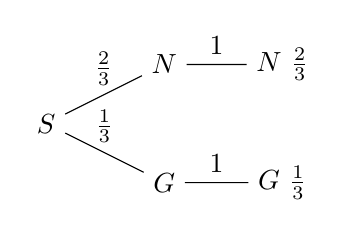
\begin{tikzpicture}[grow=right]
    \node {$S$}
        child
        {
            node {$G$}
            child
            {
                node {$G\ \frac{1}{3}$}
                edge from parent node[above] {$1$}
            }
            edge from parent node[above] {$\frac{1}{3}$}
        }
        child
        {
            node {$N$}
            child
            {
                node {$N\ \frac{2}{3}$}
                edge from parent node[above] {$1$}
            }
            edge from parent node[above] {$\frac{2}{3}$}
        };
\end{tikzpicture}\\
Ohne Wechseln
\end{minipage}
\begin{minipage}{0.45\textwidth}
\centering
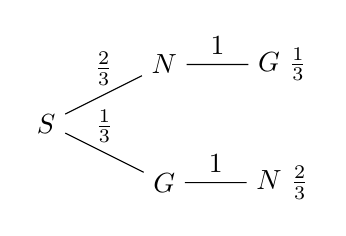
\begin{tikzpicture}[grow=right]
    \node {$S$}
        child
        {
            node {$G$}
            child
            {
                node {$N\ \frac{2}{3}$}
                edge from parent node[above] {$1$}
            }
            edge from parent node[above] {$\frac{1}{3}$}
        }
        child
        {
            node {$N$}
            child
            {
                node {$G\ \frac{1}{3}$}
                edge from parent node[above] {$1$}
            }
            edge from parent node[above] {$\frac{2}{3}$}
        };
\end{tikzpicture}\\
Mit Wechseln
\end{minipage}
\end{center}
mit Start ($S$), Gewinn ($G$) und Niete ($N$).
\subsection{Kombinatorik}
Wie bestimmt man in einer Laplace-Situation $|A|$ und $|\Omega|$?
\subsubsection{Beispiele}
\abc{
\item Sei $\Omega=A\times B$, so ist $|\Omega|=|A|\cdot|B|$ M\"unzwurf, dann W\"urfel:
\meq{A=\{\text{K},\text{Z}\},\ B=\{1,\ldots,6\}.}
\item Urne mit $N$ durchnummerierten Kugeln. Wir ziehen davon nacheinander ohne Zur\"ucklegen $k$ Kugeln (Reihenfolge wird ber\"ucksichtigt):
\meq{|\Omega|=N(N-1)\ldots(N-k+1)=\frac{N!}{(N-k)!}.}
\item Zahlenlotto ``6 aus 49'', wie b) ohne R\"ucksicht auf Reihenfolge:
\meq{|\Omega|=\frac{N!}{(N-k)!}\cdot\frac{1}{k!}.}
\item Anzahl der Anagramme von \ttt{MISSISSIPPI}.
\meq{|\Omega|=\frac{11!}{\ubr{4!}{\ttt{I}}\ubr{4!}{\ttt{S}}\ubr{2!}{\ttt{P}}}.}
}
\section{Allgemeine Wahrscheinlichkeitsr\"aume}
Wir werden das 3. Axiom von Kolmogorov anpassen:
\meq{\PP(\bigcup_{j=1}^\infty A_j)=\sum_{j=1}^\infty\PP(A_j),\ \text{falls}\ A_j\cap A_k=\emptyset,\ \forall j\neq k.}
Schwieriger ist die anpassung des Definitionsbereiches von $\PP$. Warum ist das n\"otig? Betrachte das Beispiel ``Gl\"ucksrad''.

\pickl{22.04.2024}
\subsubsection{Lemma}
Es gibt kein translationsinvariantes Wahrscheinlichkeitsma\ss{} auf $\PP([0,2\pi[)$.
\subsubsection{Beweis}
WA: Es gibt ein solches $\PP$.
\\~\\
Wir zerlegen nun $[0,2\pi[$ in \"uberabz\"ahlbar viele abz\"ahlbare Teilmengen:
\meq{a~b:\LRA a-b\in\QQ.}
Dies definiert \"Aquivalenzklassen, diese dienen zur Zerlegung von $[0,2\pi[$:
\bul{
\item $\{0,\frac{1}{2},\frac{1}{3},1,\ldots\}$,
\item $\{\sqrt{2},\sqrt{2}+\frac{1}{2},\ldots\}$,
\item $\{\pi,\pi+\frac{1}{2},\ldots\}$,
\item \ldots
}
Wir w\"ahlen aus jeder \"Aquivalenzklasse einen Representanten $\leftarrow\{0,\sqrt{2},\pi,\ldots\}$. $R$ ist nat\"urlich \"uberabz\"ahlbar. F\"ur jedes $q\in[0,2\pi[\cap\QQ$ definieren wir
\meq{R_q:=\{r+q,\ r\in R\}=R+q.}
Nach Annahme der Translationsinvarianz ist
\meq{\PP(R_q)=\PP(R),\ \forall q\in[0,2\pi[\cap\QQ.}
Es gilt:
\meq{{}[0,2\pi[\ \subseteq\ \bigcup_{\mathclap{q\in]-2\pi,2\pi[\cap\QQ}}\ R_q\subset\ ]-2\pi,4\pi[.}
$\RA$ da $\PP([0,2\pi[)=1$, gilt, dass
\meq{
    &\PP(\bigcup_{\mathclap{q\in]-2\pi,2\pi[\cap\QQ}}R_q)\geq1.\\
    \RA\ &\sum_{\mathclap{j\in]-2\pi,2\pi[}}\PP(R)\geq1\\
    \RA\ &\PP(R)\neq0,
}
aber falls der Inhalt $\PP(R)>0$, folgt, dass das Intervall $]-2\pi,4\pi[$ unendlichen Inhalt hat. Dieses \"uberdeckt jedoch $[0,2\pi[$ dreimal. $\lightning$
\subsection{Ereignisraum}
Wir schr\"anken den Definitionsbereich von $\PP$ ein, um solch problematische Mengen zu umgehen. 
\subsubsection{$\sigma$-Algebra}
Sei $\Omega$ eine Menge. Eine $\sigma$-Algebra bzgl. $\Omega$ ist eine Teilmenge von $\PP(\Omega)$ mit:
\abc{
\item $\Omega\in\Acal$,
\item $A\in\Acal\RA A^C\in\Acal$,
\item Sei $(A_n)_{n\in\NN}\subset\Acal\RA\bigcup_{n=1}^\infty A_n\in\Acal$.
}
\subsubsection{Beispiele}
\abc{
\item $\PP(\Omega)$, sowie $\{\emptyset,\Omega\}$ ist jeweils $\sigma$-Algebra.
\item
    \bul{
    \item $\Omega=\{1,2,3,4\}$.
    \item $\Acal=\{\emptyset,\Omega,\{1,2\},\{3\},\{4\},\{3,4\},\{1,2,4\},\{1,2,3\}\}$.
    }
}
\subsubsection{Satz}
Sei $\Acal$ eine $\sigma$-Algebra bzgl. $\Omega$. Dann gilt:
\abc{
\item $\emptyset\in\Acal$,
\item abz\"ahlbare Schritte von Ereignissen sind in $\Acal$,
\item $A,B\in\Acal\RA A\setminus B\in\Acal$.
}
\subsubsection{Beweis}
\abc{
\item $\emptyset=\Omega^C\in\Acal$,
\item $\bigcap_{n=1}^\infty A_n=\left[\bigcup_{n=1}^\infty A^C_n\right]^C\in\Acal$,
\item $A\setminus B=A\cap B^C$.
}
\subsubsection{Satz}
Sei $\Omega$ eine Menge. Der Schnitt beliebiger $\sigma$-Algebren ergibt wieder eine $\sigma$-Algebra.
\subsubsection{Beweis}
Seien $\Acal_i$ f\"ur $i\in\Ical$ $\sigma$-Algebren (bzgl. $\Omega$). Z.z. $\Acal:=\bigcap_{i\in\Ical}\Acal_i$ ist $\sigma$-Algebra.
\abc{
\item $\Omega\in\Acal_i,\ \forall i\in\Ical\RA\Omega\in\Acal.$
\item Sei $E\in\Acal\RA E\in\Acal_i,\ \forall i\in\Ical\RA E^C\in\Acal_i,\ \forall i\in\Ical$.
\item Seien $(E_n)_{n\in\NN}\subset\Acal$ ($E_n\in\Acal\ \forall n\in\NN$):
\meq{
    \RA\ &E_n\in A_i,\ \forall n\in\NN, \forall i\in\Ical\\
    \RA\ &\bigcup_{n=1}^\infty E_n\in\Acal_i,\ \forall i\in\Ical\ \text{(da $\Acal_i$ $\sigma$-Algebra)}\\
    \RA\ &\bigcup_{n=1}^\infty E_n\in\Acal.
}
}
\subsubsection{Bemerkung}
Vereinigungen von $\sigma$-Algebren ergeben \trt{nicht} notwendigerweise eine $\sigma$-Algebra.
\subsubsection{Beispiel}
$\Omega=\{1,2,3\}$.
\bul{
\item $\Acal_1=\{\Omega,\emptyset,\{1,2\},\{3\}\}$,
\item $\Acal_2=\{\Omega,\emptyset,\{1,3\},\{2\}\}$,
\item $\Acal_1\cup\Acal_2=\{\Omega,\emptyset,\{1,2\},\{1,3\},\{2\},\{3\}\}\not\ni\{2\}\cup\{3\}.$
}
\subsubsection{Definition (Erzeugte $\sigma$-Algebra)}
Sei $\Omega$ eine Menge, $\Ecal\subset\Pcal(\Omega)$. Die $\sigma$-Algebra $\sigma(\Ecal)$ definiert durch
\meq{\sigma(\Ecal):=\bigcap_{\mathclap{\Acal\text{ ist $\sigma$-Alg},\ \Ecal\subset\Acal}}\Acal}
nennen wir die \trt{von $\Ecal$ erzeugte $\sigma$-Algebra}.
\subsubsection{Bemerkung}
$\sigma(\Ecal)$ ist f\"ur nichtleere $\Omega$ immer wohldefiniert und wegen Satz $\sigma$-Algebra.
\subsubsection{Korollar}
$\sigma(\Ecal)$ ist die kleinste $\sigma$-Algebra, die $\Ecal$ enth\"alt, d.h.
\abc{
\item $\Ecal\in\sigma(\Ecal)$,
\item $\forall\widetilde{\Acal}$ $\sigma$-Algebra it $\Ecal\subset\widetilde{\Acal}$, gilt $\sigma(\Ecal)\subset\widetilde{\Acal}$.
}
\subsubsection{Beweis}
\abc{
\item $\Ecal$ ist in allen $\sigma$-Algebren enthalten, \"uber die der Schnitt gebildet wird.
\item $\widetilde{\Acal}$ ist ein Kandidat f\"ur $\Acal$ in der Definition. Es wird also auch \"uber $\widetilde{\Acal}$ der Schnitt gebildet $\RA\widetilde{A}\supset\sigma(\Ecal)$.
}
\subsubsection{Beispiel}
$\Omega=\{1,2,3\},\Ecal=\{\{1,2\}\}$. $\Pcal(\Omega)$ ist $\sigma$-Algebra, enth\"alt $\Ecal$ $\Acal_1$ vom Beispiel oben ebenso. Weitere Kandidaten:
\meq{\mathcal{B}=\{\Omega,\emptyset,\{1,2\},\{3\},\{1\},\{2\},\ldots\}.}


\pickl{25.04.2024}
\subsubsection{Defintiion (Borel-$\sigma$-Algebra)}
Sei $\Omega=\RR$. Die von den offenen Teilmengen von $\RR$ erzeugte $\sigma$-Algebra hei\ss{}t \trt{Borel-$\sigma$-Algebra}. (alternative Definiton sp\"ater)
\subsection{Das Wahrscheinlichkeitsma\ss{}}
\subsubsection{Definition (Wahrscheinlichkeitsma\ss{})}
Sei $\Omega$ eine Menge, $\Acal$ $\sigma$-Algebra. Eine Abbildung $\PP\colon\Acal\to\RR$ hei\ss{}t \trt{Wahrscheinlichkeitsma\ss{}} $:\LRA$
\abc{
\item $\PP(\Omega)=1$,
\item $\PP(A)\geq0,\ \forall A\in\Acal$,
\item $\PP(\bigcup_{n=1}^\infty A_n)=\sum_{n=1}^\infty\PP(A_n)$, falls $A_n\in\Acal,\ A_n\cap A_m=\emptyset\ \forall n\neq m$.
}
\subsubsection{Bemerkung}
Satz vom Gegenereignis, $\PP(\emptyset)=0$ und $\PP(A\cup B)=\PP(A)+\PP(B)-\PP(A\cap B)$ gilt weiterhin.
\subsubsection{Definition und Satz (Bedingte Wahrscheinlichkeit)}
Sei $(\Omega,\Acal,\PP)$ ein Wahrscheinlichkeitsraum, d.h. $\Omega$ Menge, $\Acal$ zugeh\"orige $\sigma$-Algebra, $\PP\colon\AA\to\RR$ Wahrscheinlichkeitsma\ss{}.
\\~\\
Sei $A\in\Acal$ mit $\PP(A)\neq0$. Dann ist das auf $A$ \trt{bedingte Wahrscheinlichkeitsma\ss{}} definiert durch
\meq{\PP_A(B)=\frac{\PP(A\cap B)}{\PP(A)}.}
\subsubsection{Beweis}
(dass dies ein Wahrscheinlichkeitsma\ss{} ist):
\abc{
\item $\PP_A(\Omega)=\frac{\PP(A\cap\Omega)}{\PP(A)}=\frac{\PP(A)}{\PP(A)}=1.$
\item Z\"ahler $\geq0$, Nenner $>0$ $\RA$ Behauptung.
\item 
\meq{
    \PP_A(\bigcup_{n=1}^\infty A_n)&=\frac{\PP(A\ \cap\ \bigcup_{n=1}^\infty A_n)}{\PP(A)}\ (A_n\cap A_m=\emptyset,\ n\neq m)\\
    &=\frac{\PP(\bigcup_{n=1}^\infty\obr{(A_n\cap A)}{paarweise disjunkt})}{\PP(A)}\\
    &=\frac{\sum_{n=1}^\infty\PP(A_n\cap A)}{\PP(A)}\\
    &=\sum_{n=1}^\infty\PP_A(A_n).
}
}
\subsubsection{Definition (Unabh\"angigkeit)}
Zwei Ereignisse $A,B$ hei\ss{}en (stochastisch) \trt{unab\"angig} $:\LRA$
\meq{\PP(A\cap B)=\PP(A)\cdot\PP(B)}.
\subsubsection{Bemerkung}
$A$ unabh\"angig von $B$ $\RA$ $\PP_A(B)=\PP(B)$ (falls $\PP(A)\neq0$).


\end{document}

